\documentclass[aspectratio=169,10pt]{beamer}
% Course-local adaptation of the copied Sorbonne Beamer reference assets.
% The files in template/assets/ are preserved verbatim from the reference copy.
\usepackage[T1]{fontenc}
\usepackage[utf8]{inputenc}
\usepackage{lmodern}
\usepackage{amsmath,amssymb,mathtools}
\usepackage{booktabs}
\usepackage{graphicx}
\usepackage{tikz}
\usetikzlibrary{arrows.meta,positioning,calc}
\usepackage{ragged2e}
\usepackage{hyperref}
\definecolor{bleu}{RGB}{0,129,188}
\definecolor{rouge}{RGB}{238,50,78}
\definecolor{orange}{RGB}{255,100,0}
\definecolor{vert}{RGB}{0,157,87}
\definecolor{dp}{RGB}{181,73,60}
\usetheme{Frankfurt}
\useoutertheme[subsection=false,shadow]{miniframes}
\usepackage{template/assets/beamercolorthemeEwen}
\usepackage{template/assets/beamerouterthemeEwen}
\usepackage{template/assets/beamerhighlight}
\usefonttheme{serif}
\setbeamerfont{title like}{shape=\scshape}
\setbeamerfont{frametitle}{shape=\scshape}
\setbeamercolor{frametitle}{fg=dp,bg=white}
\setbeamercolor{structure}{fg=black}
\setbeamercolor{alerted text}{fg=dp}
\setbeamertemplate{navigation symbols}{}
\setbeamertemplate{items}[triangle]
\setbeamertemplate{footline}{%
  \leavevmode\hbox{\begin{beamercolorbox}[wd=1\paperwidth,ht=2.25ex,dp=1ex,center]{title in head/foot}
  \hfill\hspace*{8em}\insertshorttitle\hspace*{2em}\insertframenumber{} / \inserttotalframenumber\hspace*{1ex}
  \end{beamercolorbox}}\vskip0pt}
\newcommand{\key}[1]{\textcolor{dp}{\textbf{#1}}}
\AtBeginSection[]{\begin{frame}{Plan}\tableofcontents[currentsection,hideallsubsections]\end{frame}}

\title[BTM -- Session 1]{Modern Business Cycle Theory}
\subtitle{Measurement, expectations and a consumption--saving model}
\author[Gauthier Vermandel]{Gauthier Vermandel}
\institute{Paris-Dauphine -- PSL}
\date{5 November 2026}
\begin{document}
\begin{frame}\titlepage\end{frame}
\begin{frame}{Session objective}
\begin{itemize}
\item Move from observed macroeconomic series to a disciplined notion of a business cycle.
\item Use a simple intertemporal model to connect shocks, expectations and aggregate fluctuations.
\item Prepare the approximation tools used throughout the course.
\end{itemize}
\vfill\key{Handout:} Session 1 \quad \key{Code:} \texttt{code/session1/}
\end{frame}
\section{What is a cycle?}
\begin{frame}{Observed output combines several objects}
\centering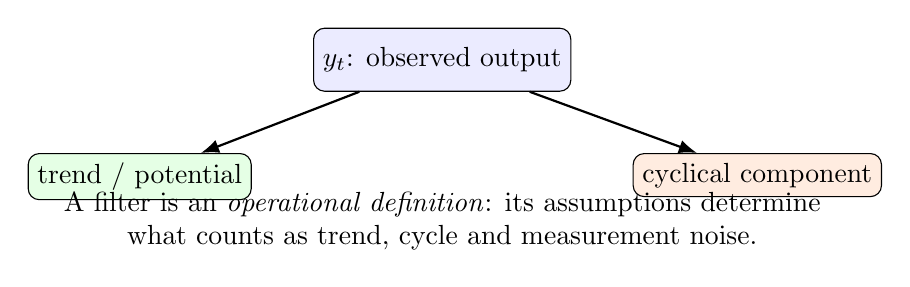
\begin{tikzpicture}[node distance=1.1cm,>=Latex]
\node[draw,rounded corners,fill=blue!8,minimum width=3.0cm,minimum height=.8cm] (y) {$y_t$: observed output};
\node[draw,rounded corners,fill=green!10,below left=of y,minimum width=2.8cm] (trend) {trend / potential};
\node[draw,rounded corners,fill=orange!12,below right=of y,minimum width=2.8cm] (cycle) {cyclical component};
\draw[->,thick] (y) -- (trend); \draw[->,thick] (y) -- (cycle);
\node[below=1.15cm of y,align=center] {A filter is an \emph{operational definition}: its assumptions determine\\what counts as trend, cycle and measurement noise.};
\end{tikzpicture}\end{frame}
\begin{frame}{Three questions before filtering}
\begin{enumerate}\item What frequency range corresponds to the economic question?\item Is the trend deterministic, stochastic or model based?\item What happens at the sample endpoints and after revisions?\end{enumerate}
\vfill\begin{block}{Course principle}Filtering is not neutral preprocessing. It is part of the empirical model and must be documented.\end{block}
\end{frame}
\section{A dynamic benchmark}
\begin{frame}{A consumption--saving problem}
\begin{columns}[T]\begin{column}{.52\textwidth}Household choice:
\[\max_{\{c_t,a_{t+1}\}}\; \mathbb E_0\sum_{t\geq0}\beta^t u(c_t)\]
subject to \[c_t+a_{t+1}=y_t+(1+r_t)a_t.\]
\end{column}\begin{column}{.43\textwidth}\begin{itemize}\item \(\beta\): patience\item \(a_t\): assets carried into \(t\)\item \(r_t\): intertemporal price\item \(y_t\): stochastic income\end{itemize}\end{column}\end{columns}
\vfill\key{Economic force:} households smooth consumption across states and dates.\end{frame}
\begin{frame}{Euler equation: the key restriction}
\[u'(c_t)=\beta\,\mathbb E_t\left[(1+r_{t+1})u'(c_{t+1})\right].\]
\begin{itemize}\item Current consumption trades off against expected marginal utility tomorrow.\item Expectations are endogenous: beliefs concern future equilibrium objects.\item Estimation later asks which parameters make these restrictions fit the data.\end{itemize}
\end{frame}
\section{From nonlinear model to usable system}
\begin{frame}{A reproducible workflow}
\centering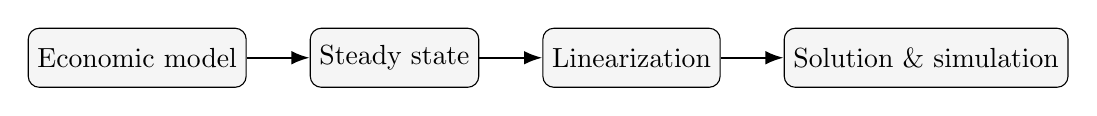
\begin{tikzpicture}[node distance=.8cm,>=Latex,every node/.style={draw,rounded corners,align=center,minimum height=.75cm,fill=gray!8}]
\node (m) {Economic model};\node[right=of m] (s) {Steady state};\node[right=of s] (l) {Linearization};\node[right=of l] (q) {Solution \& simulation};
\draw[->,thick] (m)--(s);\draw[->,thick] (s)--(l);\draw[->,thick] (l)--(q);\end{tikzpicture}
\vfill\begin{itemize}\item Keep the nonlinear model and the approximation separate.\item Check residuals and units before interpreting an impulse response.\end{itemize}\end{frame}
\begin{frame}{First-order approximation}
For a system \(F(x_{t+1},x_t,x_{t-1},\varepsilon_t)=0\), expand around the deterministic steady state:
\[F_x\widehat x_{t+1}+F_y\widehat x_t+F_z\widehat x_{t-1}+F_\varepsilon\varepsilon_t\simeq0.\]
\begin{block}{Why it matters}Linear systems make expectations, filtering and likelihood evaluation computationally tractable.\end{block}\end{frame}
\section{Takeaways}
\begin{frame}{Takeaways and preparation}\begin{itemize}\item Business-cycle facts depend on measurement choices.\item Dynamic macroeconomic models express restrictions through Euler equations and expectations.\item Linearization supplies the state-space objects used in Sessions 2--4.\end{itemize}\vfill\key{Before Session 2:} run \texttt{toy\_model.m} and inspect the model, steady state and simulated paths.\end{frame}
\end{document}
